\documentclass[a4paper, 12pt]{article}
\usepackage[T2A]{fontenc}
\usepackage[utf8]{inputenc}
\usepackage[english,russian]{babel}
\usepackage{amsmath, amsfonts, amssymb, amsthm, mathtools, misccorr, indentfirst, multirow}
\usepackage{wrapfig}
\usepackage{graphicx}
\usepackage{subfig}
\usepackage{adjustbox}
\usepackage{pgfplots}

\usepackage{geometry}
\geometry{top=20mm}
\geometry{bottom=20mm}
\geometry{left=20mm}
\geometry{right=20mm}
\newcommand{\angstrom}{\textup{\AA}}

\begin{document}
	\title{Лабораторная работа №4.2\\Исследование энергетического спектра $\beta$-частиц и определение их максимальной энергии при помощи магнитного спектрометра}
	\author{Нехаев Александр 654гр.}
	\maketitle
	\tableofcontents
	\section{Введение}
	Бета-распад это самопроизвольное преваращение ядер, при котором их массовове число не изменяется, а заряд изменяется на единицу. В данной работе мы будем иметь дело с электронным распадом:
		\begin{equation}
		    _{Z}^{A}X \rightarrow _{Z+1}^{A}X + e^{-} + \widetilde{\nu}
		\end{equation}
		Освобождающаяся в результате распада энергия делится между исходным ядром, электроном и нейтрино. При этом доля энергии, уносимая ядром крайне мала, так что вся энергия делится между нейтрино и электроном. Поэтому электроны могут иметь любую энергию от нулевой до некоторой макимальной энергии, высвобождаемой при распаде.
		
		Вероятность $d\omega$ того, что электрон вылетит с имульсом $d^3p$, а нейтрино с импульсом $d^3k$ равна произведению этих дифференциалов, но мы должны учесть также закон сохранения энергии.
		\begin{equation}
		    E_e - E - ck = 0
		\end{equation}
		Энергия электрона связана с импульсом обычным образом:
		\begin{equation}
		    E = c\sqrt{p^2 + m^2c^2} -mc^2
		\end{equation}
		Таким образом, вероятность $d\omega$ принимает вид:
		\begin{equation}
		    d\omega = D\delta(E_e-E-ck)d^3pd^3k = D\delta(E_e-E-ck)p^2d pk^2d kd\Omega_ed\Omega_{\widetilde{\nu}}
		\end{equation}
		D можно считать с хорошей точностью константой. В этом случае можно проинтегрировать по всем углам и по абсолютному значению импульса нейтрино. В этом случае $\delta$-функция исчезнет, а $ck$ всюду заменится на $E_e-E$. После умножения на полное число распадов выражение примет вид:
		\begin{equation}
		    d N = \frac{16\pi^2N_0}{c^2} D p^2\left(E_e-E\right)^2d p
		\end{equation}
		В нерелятивистском случае выражение упрощается и принимает вид:
		\begin{equation}
			\frac{d N}{d E} \simeq \sqrt{E}(E_e - E)^2
		\end{equation} 
		\begin{figure}[h!]
			\centering
			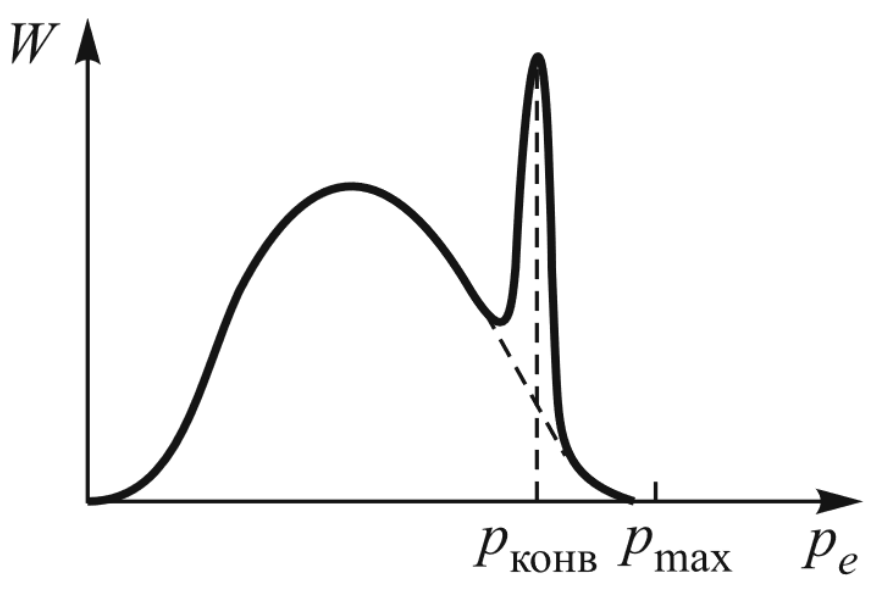
\includegraphics[width=0.6\linewidth]{pic1}
			\caption{Форма спектра $\beta$-частиц при разрешенных переходах}
		\end{figure}
		\section{Экспериментальная установка}
		Энергия определяется с помощью $\beta$-спектрометров. В работе используется магнитный спектрометр с короткой линзой.
		\begin{figure}[!htb]
			\centering
			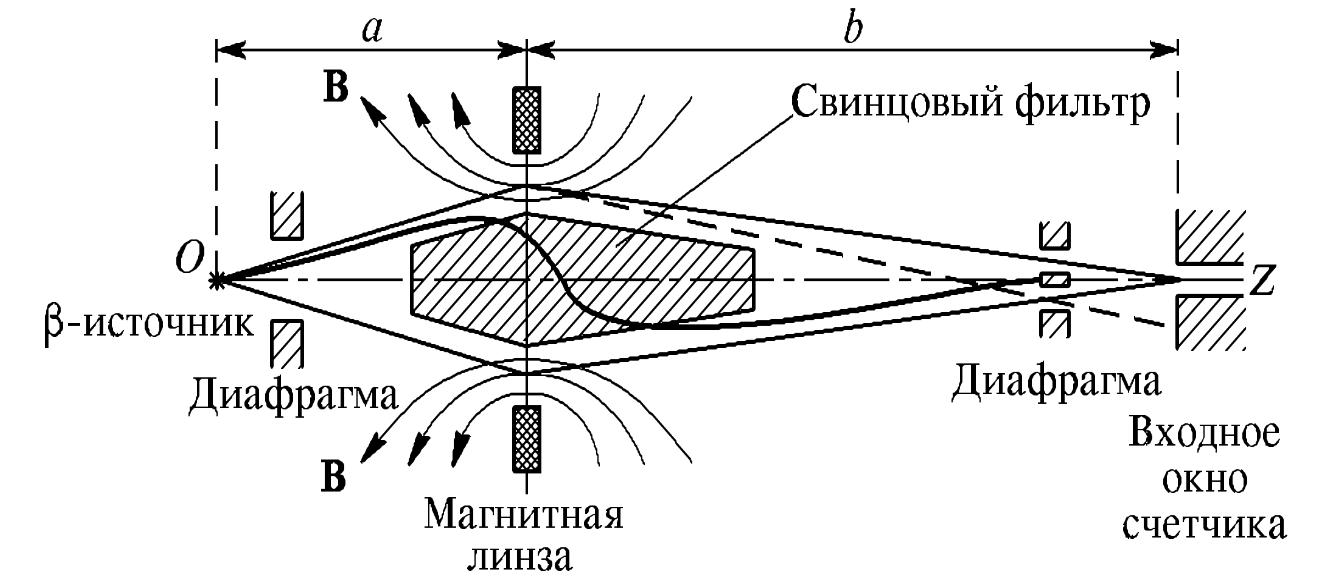
\includegraphics[width=0.8\linewidth]{pic2}
			\caption{Схема $\beta$-спектрометра с короткой линзой}
		\end{figure}
		Как показывает расчет, для заряженных частиц тонкая катушка эквивалентна линзе:
		\begin{equation}
			\frac{1}{f} \simeq \frac{I^2}{p_e^2}
		\end{equation}
		При заданной силе тока на входное окно счетчика собираются электроны с определенным импульсом.
		\section{Ход работы}
		Снимем точки $\beta$-спектра. Фоновое излучение равно $N_b = 0.8098$. C учетом этого пересчитаем число частиц, зарегистрированных счетчиком.
		\begin{table}[!htb]
			\centering
			\begin{tabular}{|c|c|c|c|c|c|c|}
				\hline
				\# & $J$, A & $N$ & $N-N_b$ & $p$, кэВ/с & $T$, кэВ & mkFermi\\
				\hline
				1 & 0.00 & 0.880 & 
				\hline
			\end{tabular}
		\end{table}
\end{document}